\documentclass[]{article}
%opening
\title{Writeup Document}
\author{Alex Miller}
\addtolength{\oddsidemargin}{-.875in}
\addtolength{\evensidemargin}{-.875in}
\addtolength{\textwidth}{1.75in}
\addtolength{\topmargin}{-.875in}
\addtolength{\textheight}{1.75in}
\setcounter{secnumdepth}{0}
\usepackage{cancel}
\usepackage{amssymb}
\usepackage{amsmath}
\usepackage{hyperref}
\usepackage{graphicx}
\graphicspath{ {./} }
\usepackage[ruled,vlined, linesnumbered]{algorithm2e}
\DontPrintSemicolon


\begin{document}
\maketitle

\section{Changes}
\subsection{Changes to the design}
I have made the following addresses changes to my project's design, broken down by module:
\begin{itemize}
	\item Top level modules (serial.c and parallel.c)
	\begin{itemize}
		\item I modified serial.c and parallel.c to take in an optional flag denoting that the programs should be run in "correctness testing" mode. In this mode, $chksum\_serial()$ and $chksum\_parllalel()$ would not dispatch packets from $n$ sources for $M$ seconds, but $n * M$ packets total. The values these functions would return (with this flag specified) would not be throughput numbers but amalgamated checksums, as described in assignment 2.
	\end{itemize}
	\item Algorithm implementation level (chksum.c)
	\begin{itemize}
		\item I modified both  $chksum\_serial()$ and $chksum\_parallel()$ to take in the additional flag denoting whether they should generate checksums in correctness testing mode or not.
		\\\\
		If so, the dispatchers for these functions would not rely on a timed approach to halting packet generation, but would instead halt themselves and their threads after generating $M * n$ packets. The long integer returned by these methods would not represent their respective throughputs, but amalgamated checksums.
		\\\\
		Threads launched by the parallel dispatcher would not tally throughput for queues but amalgamated checksums instead. This requires the definition of the following worker methods:
		\begin{itemize}
			\item $void$ $*L\_worker\_test(void$ $*args)$
			\item $void$ $*H\_worker\_test(void$ $*args)$ 
			\item $void$ $*A\_worker\_test(void$ $*args)$
		\end{itemize}
		all of which would implement the behaviors of their namesakes, but instead record amalgamated checksums and not mere throughput. These methods would deviate from their original versions in that they generate amalgamated checksums and only exit once all queues are empty and the closing of the system is signaled. However, the $A\_worker\_test()$ method has the problem that it can't necessarily tell when \textit{all} queues are empty. As such, when indicated, $clear\_queue$ (discussed below) will be responsible for generating returning the amalgamated checksum of any packets left in a queue upon cleanup, and adding that checksum to $chksum\_parallel()$'s return value. This will insure that, if $A\_worker\_test$ isn't able to reach all packets enqueued by the dispatcher, that it at least generated the correct checksums for all packets it was able to reach.
		\\\\
		$chksum\_parallel()$ would be responsible for setting $worker\_method$ to one of these functions when specified by the correctness testing flag.
		\item My original design for both the serial and parallel dispatchers utilized a scheme in which each would repeatedly calculate and check whether they had surpassed the allotted time limit. Once written, however, this method seemed bulky and to incur no small amount of increased overhead and complexity within the packet dispatching loops.
		\\
		Now, rather than having the dispatching threads calculate time intervals themselves, they both call the new method $start\_timed\_flag()$, which takes in two arguments:
		\begin{itemize}
			\item volatile bool *done : a volatile pointer to a malloced flag
			\item int M : a integer specifying a number of milliseconds
		\end{itemize}
		This method spawns a new thread that sleeps for $M$ milliseconds before setting the value pointed to by $done$ to $true$. The method than detaches the spawned thread and returns.
		\\
		Dispatching sections can then just operate so long as the value pointed to by $done$ is $false$. In $chksum\_serial()$, this value is allocated before the test is run. In $chksum\_parallel$, this value is allocated in the $create\_queue\_pool()$ method and pointed to by all $packet\_queue\_t$ instances in the queue pool.
		\\
		This method does incur the extra overhead of managing an additional thread, which may complicate performance analysis. However, as that thread's primary task is sleeping, the effect should be negligible.
		\item I also steamlined the behavior defined by the Awesome load balancing strategy:
		\begin{itemize}
			\item Within an infinite while loop, the thread attempts to acquire a queue's associated lock with it's $trylock()$ method.
			\item If it succeeds, the thread waits to enter the critical section:
			\begin{itemize}
				\item The thread attempts to dequeue from the queue and binds the result to a pointer called $packet$.
				\item The thread then unlocks the queue's lock
				\item If $packet \neq NULL$, then the thread generates a checksum for the packet and frees it.
				\item At this point, if the thread has been signaled to close, it returns
				\item Otherwise, it atomically increments the queue's $through\_count$ counter
			\end{itemize}
			\item Once it has either attempted to acquire the lock and failed or has exited the critical section, the thread checks if it has been signalled to close. If it has it returns. Otherwise, the thread moves onto the next queue.
		\end{itemize}
	\end{itemize}
	\item Queue data structure (queue.c)
	\begin{itemize}
		\item My original declaration of my queue-pool initialization method was as follows:
		\\\\
		\textit{packet\_queue\_t *create\_queue\_pool(int num\_q, int D, char L) : allocate an array of $num\_q$ packet\_queue\_t structs, each of depth $D$. Each queue should have a lock of type $L$ associated with it. If $L$ does not specify a char code for a valid lock (if L is not t, p, m, or a), then no locks are allocated.}
		\\\\
		This method is now declared as:
		\\\\
		packet\_queue\_t *create\_queue\_pool(int num\_q, int D, char L, int n) : allocate an array of $num\_q$ packet\_queue\_t structs, each of depth $D$. Each queue should have a lock of type $L$ associated with it. If $L$ does not specify a char code for a valid lock (if L is not t, p, m, or a), then no locks are allocated. Each lock in the queue pool will be initialized to work with $n$ total threads.
		\item My implementation also now includes the method:
		\\\\
		long clear\_queue(packet\_queue\_t *Q, bool correct) 
		\\\\
		This method frees any packets in a queue -- it is used to cleanup allocated system resources. If $correct = true$, then it also generate an amalgamated checksum for the packets left in a queue and returns this value. Otherwise it merely returns $0$ 
	\end{itemize}
	\item Lock data structure (lock.c)
	\begin{itemize}
		\item No changes to report
	\end{itemize}
	\item Testing script (test\_script.sh)
	\begin{itemize}
		\item I neglected to state that I would vary trial numbers based on the type of packet generator specified by an experiment. Trials using a uniform packet generator will still utilize 5 trials. Trials using an exponential packet generator, however, will utilize 11 trials.
		\item Additionally, I will include another file, $correct\_test\_script.sh$, which utilizes the optional correctness testing scheme I described above. This script will verify that amalgamated checksums are consistent across $chksum\_serial()$ and $chksum\_parallel()$, for all load balancing strategies.
		\item Finally, I also want to test my Awesome load balancing on Uniform packets. I will therefore redo Experiment 2: Speedup with Uniform Load, but instead of using the HomeQueue strategy I will use my new Awesome strategy, in addition to my other tests. 
	\end{itemize}
	\item These changes are consistent with my previously stated invariants
\end{itemize}

\subsection{Changes to Test plan:}
As mentioned above, I will not try to verify if my Awesome load balancing strategy is strictly consistent with my serial implementation. As the Awesome strategy doesn't map worker threads to queue, the possibility remains that the threads exit our correctness testing implementation prior to generating checksums for all generated packets. As such, worker threads themselves might not generate an amalgamated checksum that is consistent $chksum\_serial()$. This discrepancy is mitigated by the use of $clear\_queue()$. For now, I am deeming this a sufficient test of correctness for my Awesome load balancing strategy. To desire more would mean having to alter the structure of the strategy as to make it a non-meaningful test of correctness.
\section{Results}
As of writing this, $correct\_test\_script.sh$ confirms that my implementations are consistent.
\\\\
The raw performance data for the Idle Lock Overhead and Speedup tests are stored in a folder called $HW3b/hw3b/exp\_data$. This folder contains the .csv files that describe performance data for a given experiment. overhead.csv describes the data from experiment 1. speedup.csv contains all other necessary data
\\
This data was collected by running implementations for given number of trials, calculating measurements per trial, and taking median values. As such there is no other collected data other than median speedup and throughput. That data was not recorded as it did not serve the purpose of analysis and would've have complicated my data storage scheme.
\\\\
As per how many trials I utilized; for experiments utilizing uniform packets, I used 5 trials; for experiments utilizing exponential packets, I used 11 trials.
\\\\
I took this data and plotted it using the script analyze.py. These graphs are stored in the folder $HW3b/Docs/graphs$. I will display these graphs below:
\subsection{Experiment 1: Idle Lock Overhead}
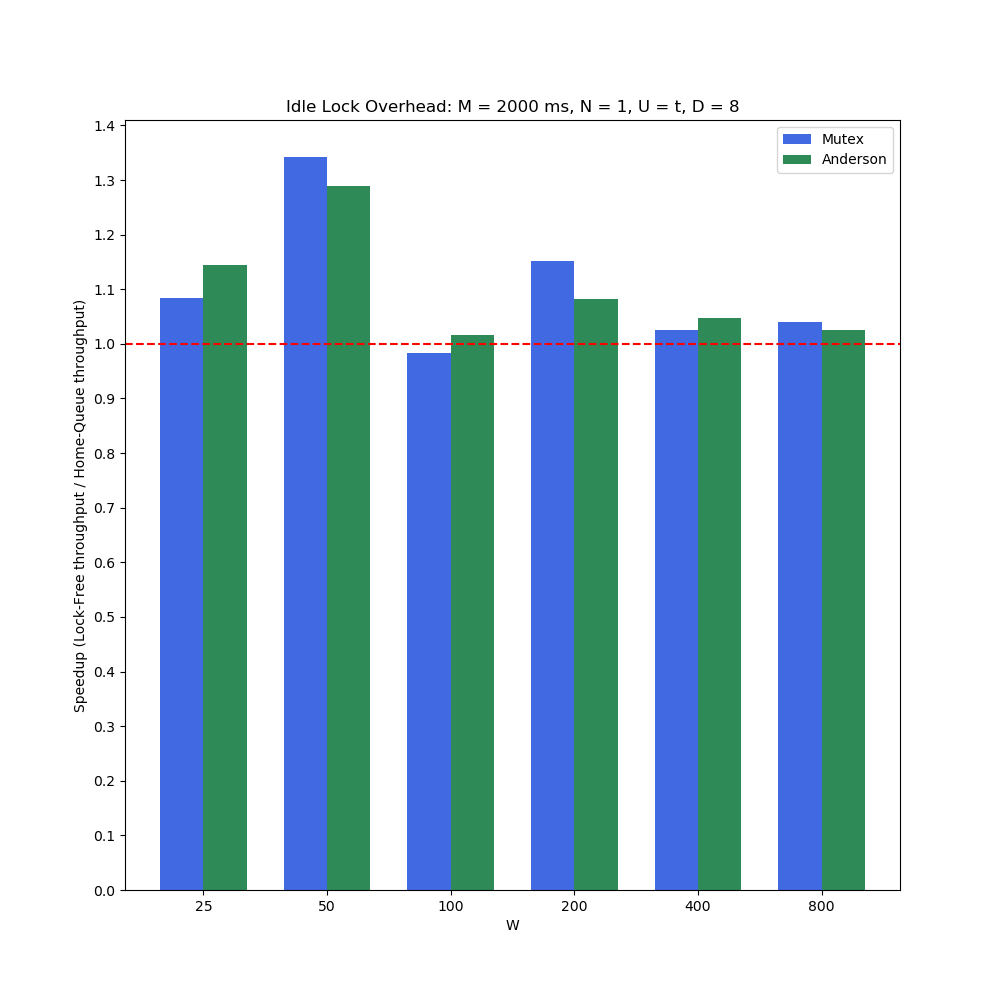
\includegraphics[scale=0.5]{graphs/overhead.png}\\
\subsection{Experiment 2: Speedup with Uniform Load}
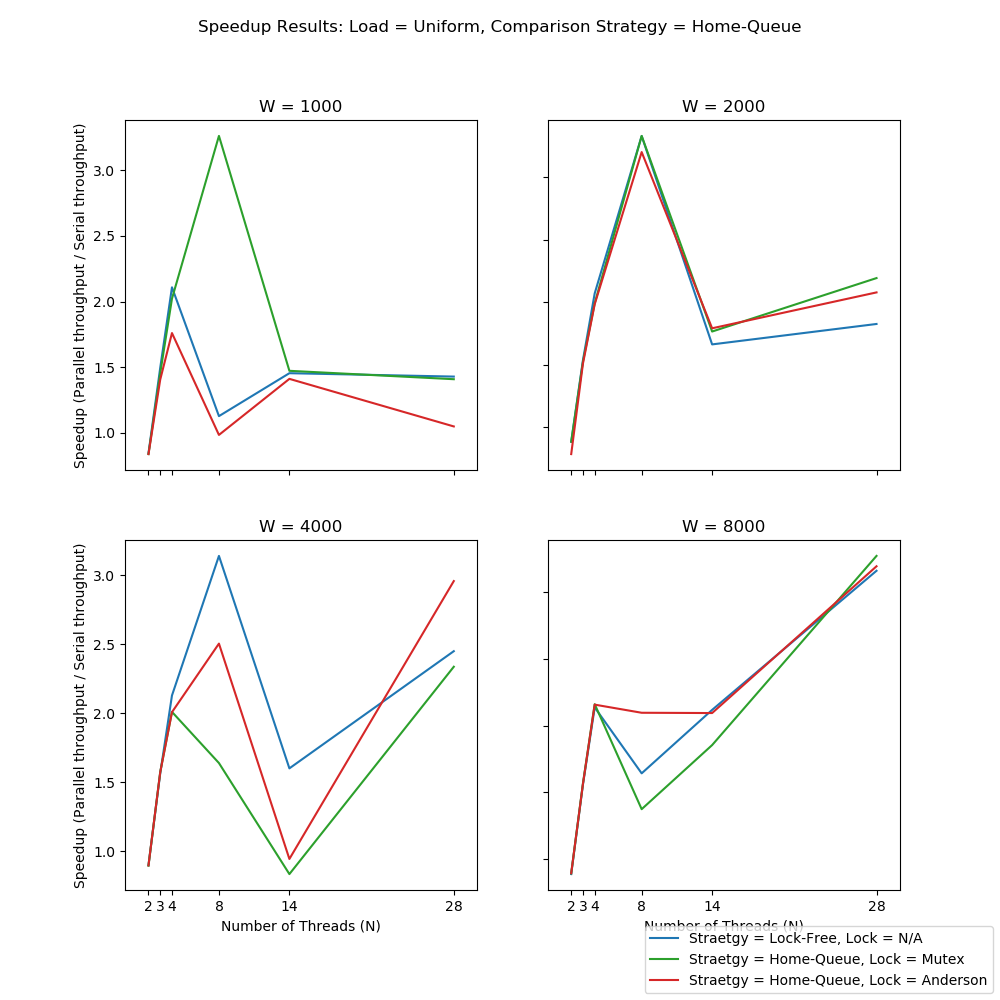
\includegraphics[scale=0.5]{graphs/speedup_t:H.png}\\
\subsection{Experiment 3: Speedup with Exponential Load}
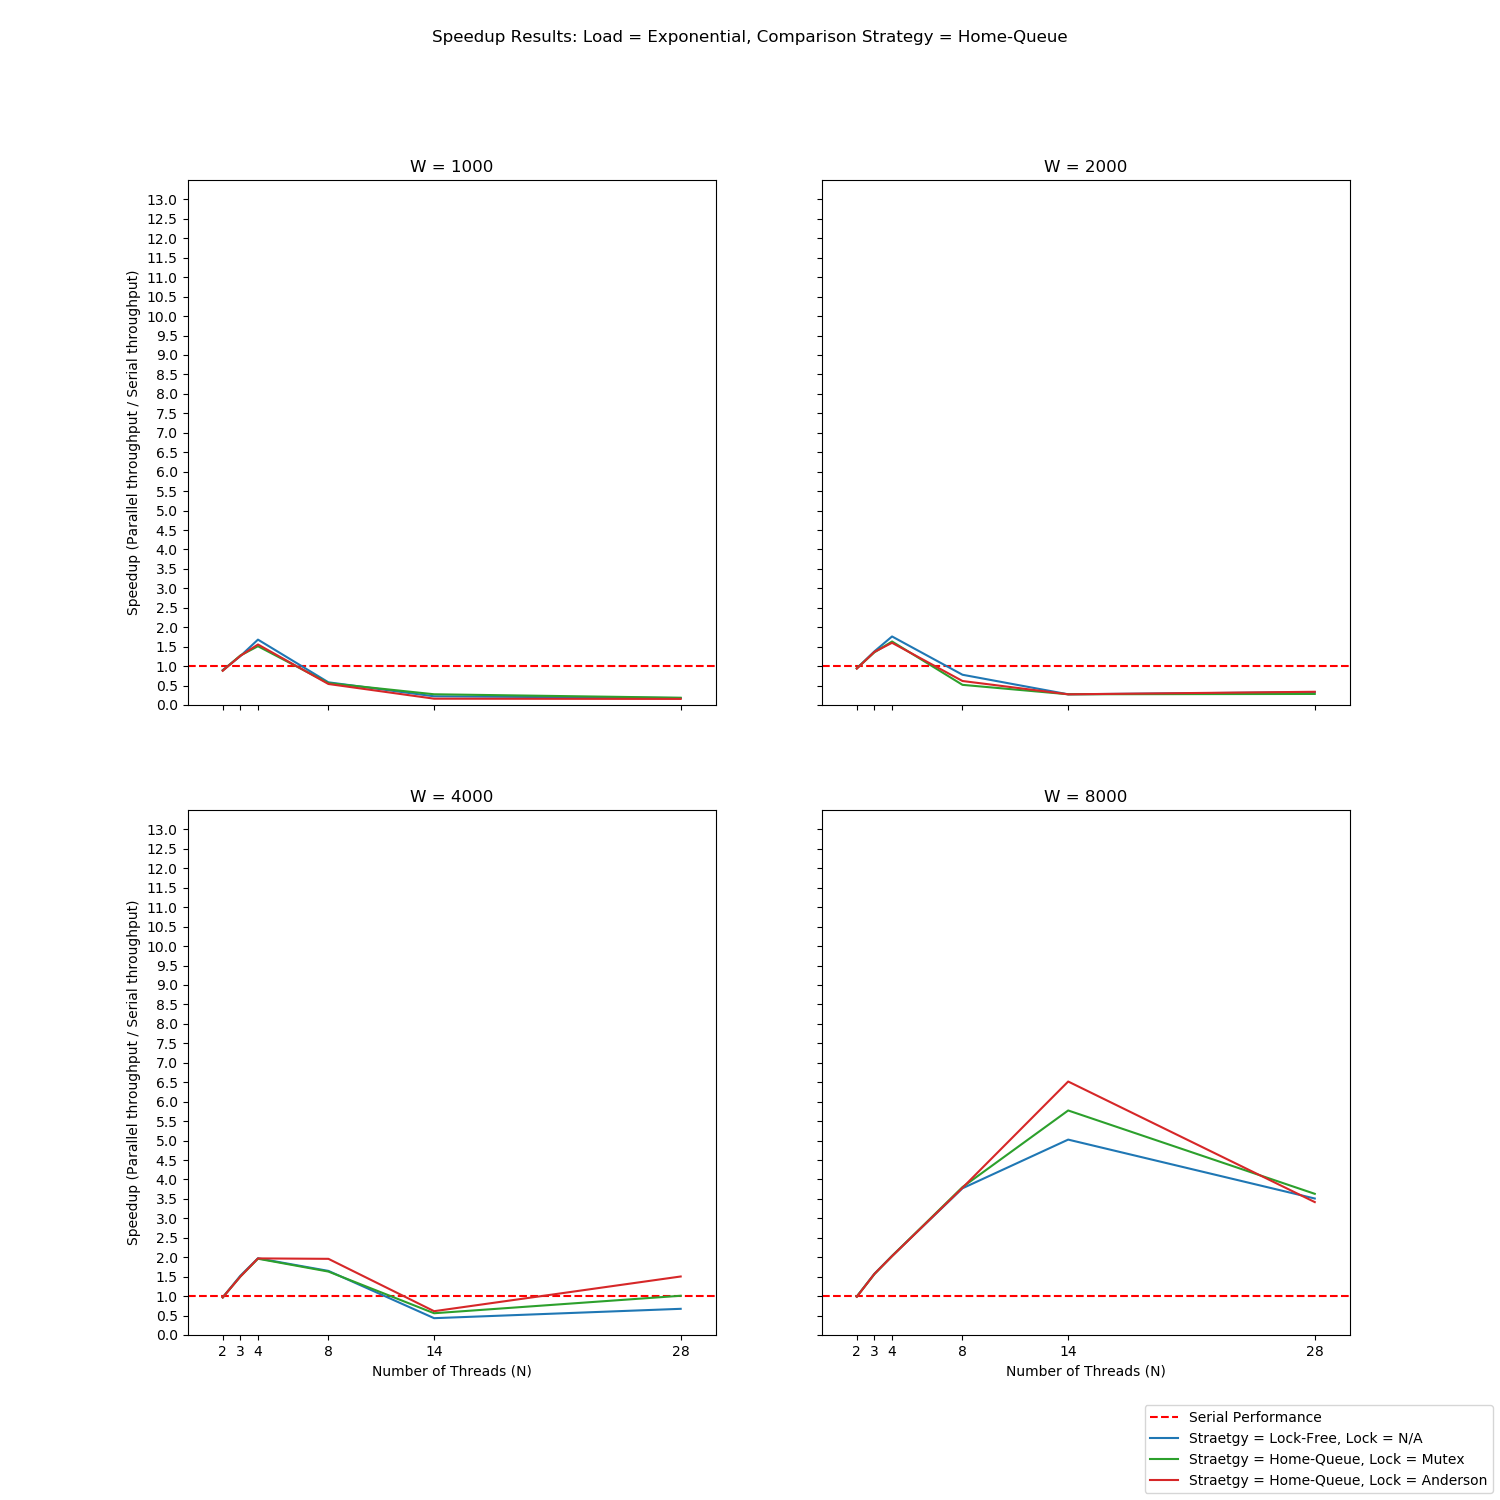
\includegraphics[scale=0.5]{graphs/speedup_f:H.png}\\
\subsection{Experiment 4: Speedup with Uniform Load (Awesome Test)}
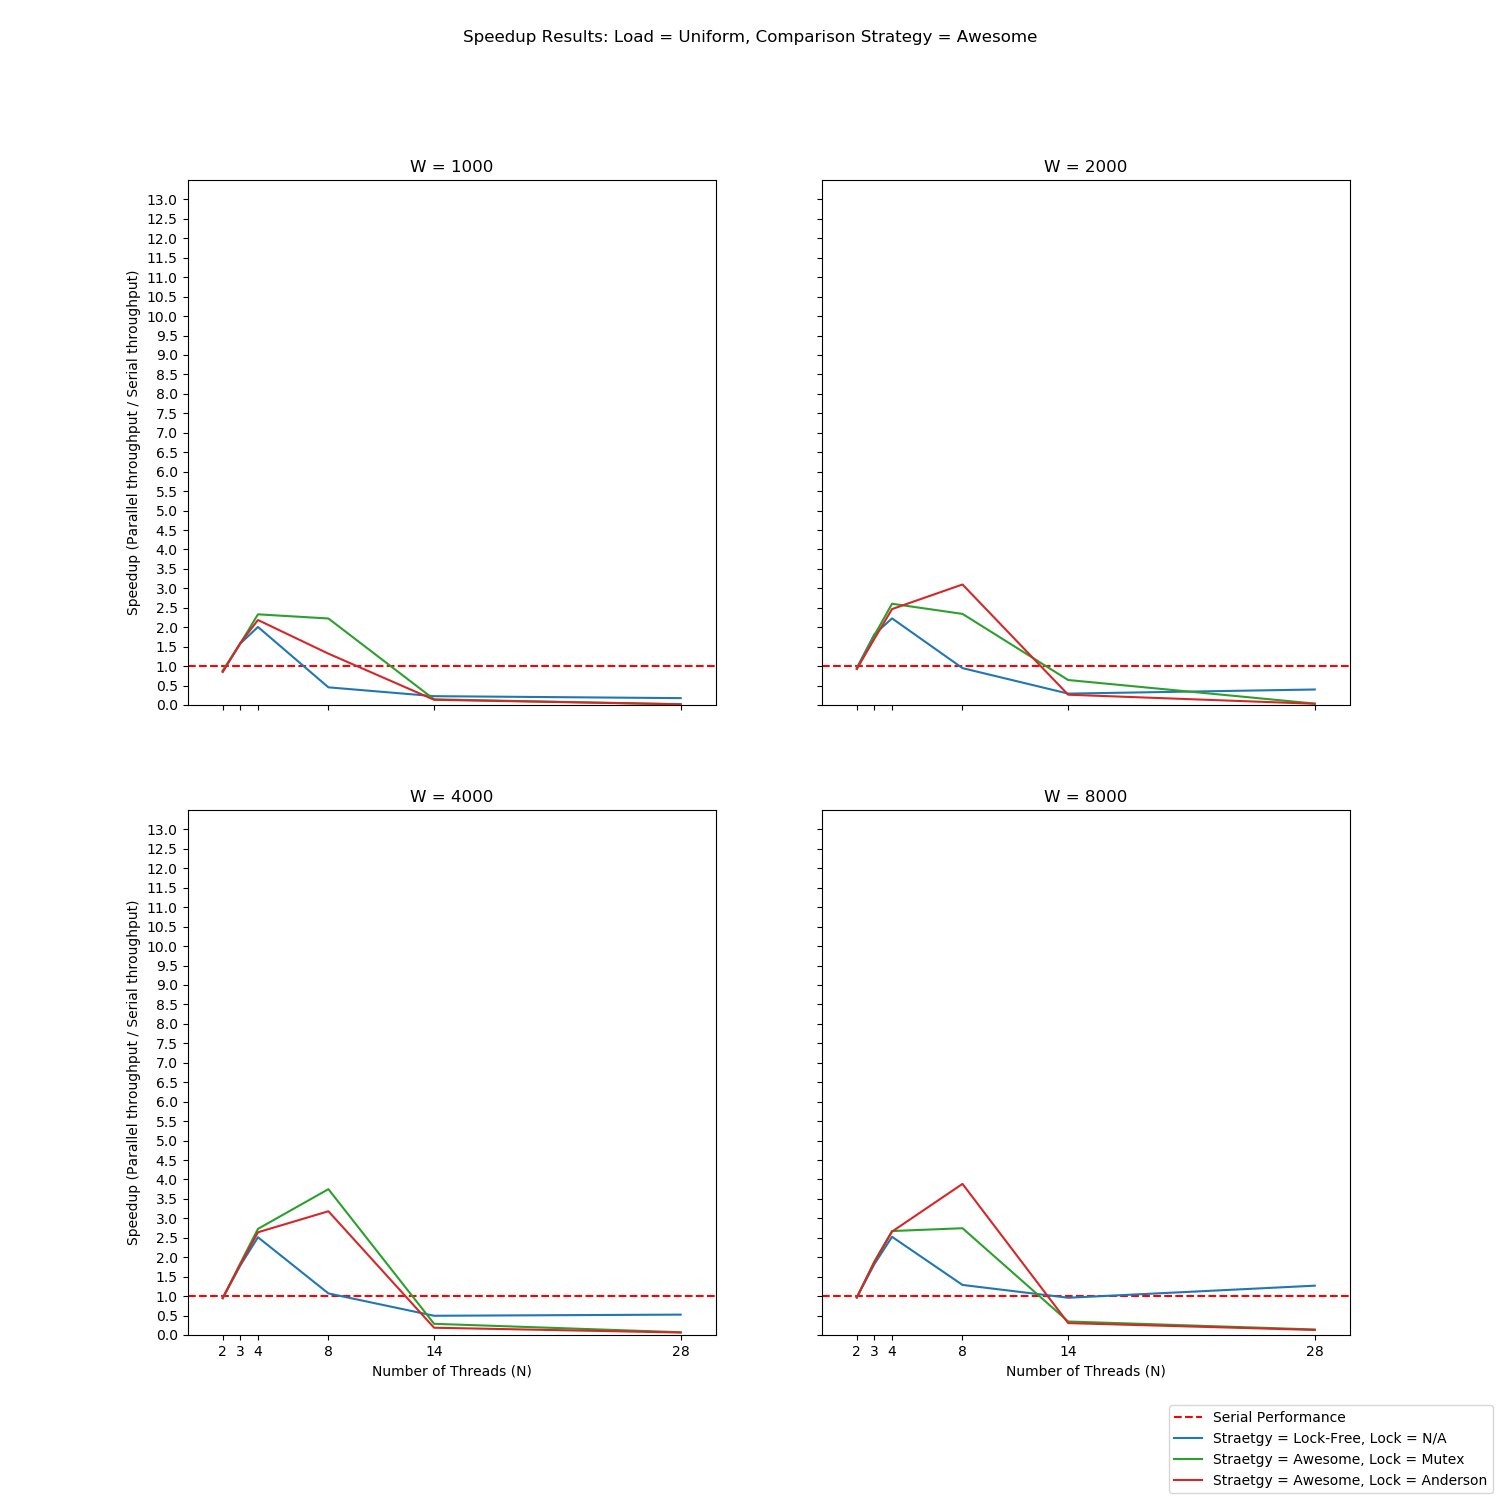
\includegraphics[scale=0.5]{graphs/speedup_t:A.png}\\
\subsection{Experiment 5: Speedup with Exponential Load (Awesome Test}
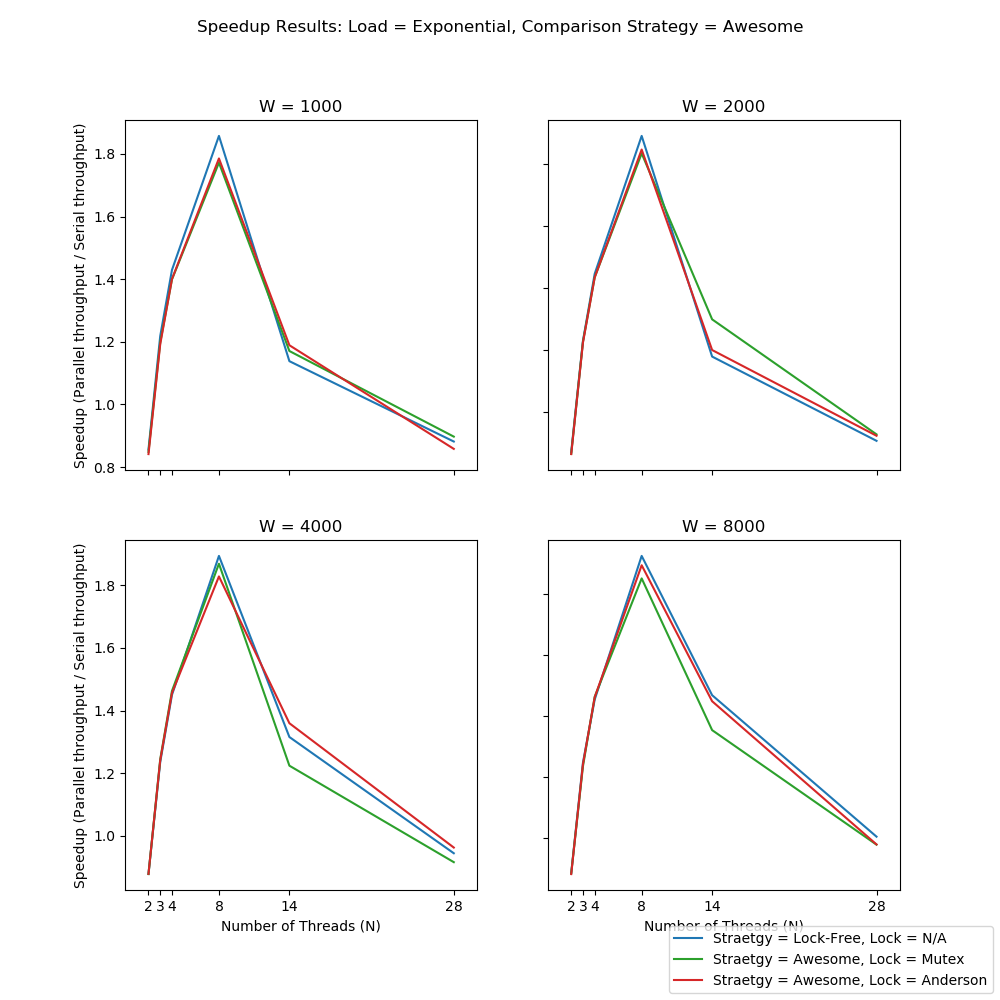
\includegraphics[scale=0.5]{graphs/speedup_f:A.png}\\

\section{Analysis}

\section{Theory}
	
\end{document}
